\documentclass[../../../../../../dd.tex]{subfiles}

\begin{document}

	\subsection{Data Tier}
	This part represent the model of the system ( using a MVC architecture ), so the class we use in this section was the representation of the information that must be stored to use the system.
	\subsubsection{Database} the database is the data structure we don't specify the classes used by this structure, all the information we store are managed by the Database Manager.
	\subsubsection{Database Manager}
	The main classes used to represent the stored data of our application are:
	\begin{itemize}
	\item{Registered User}: this class contains the information about the registered user.
	\item{Taxi Driver}: this class extends the Registered User class and represent the information about the taxi drivers 
	\item{Customer}: this class extends the Registered User class and represent the information about the customers
	\item{Zone}: this class represent the information about the zones. On this class we store also the queue of the taxi driver that are available on this specific zone.
	\item{Ride}: this class contain the general information that Ride and Request share. This abstract class follows the pattern State to represent the state of a ride. All Ride start in the state NOT\textunderscore HANDLED, then can pass in state HANDLED, then from this state can pass in the state NOT\textunderscore HANDLED.
	\item{Request}: this class extends Ride and represent the information of the requests for a ride.
	\item{Reservation}: this class extends Ride by adding information about the starting and the end position, and the time of the meeting. Adding this information we can represent the reservation in our system.
	
	\end{itemize}
	
	
	\begin{figure}[H]
				\centering
				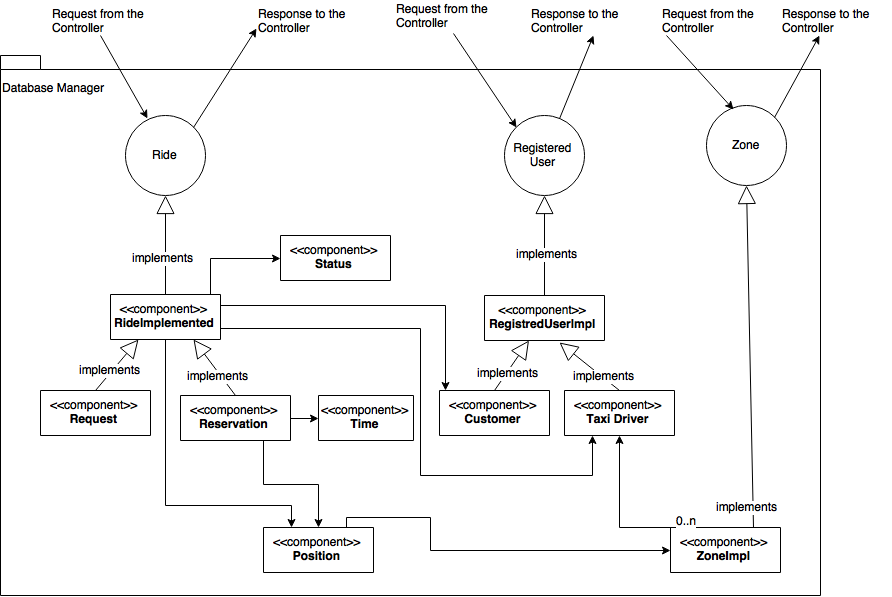
\includegraphics[width=\textwidth, scale=0.5]{../images/DataTier.png}
			\caption{Data Manager Structure}\label{fig:DBMS}
		\end{figure}
	
	
	 
\end{document}